% author: Tomas Trnka
% mail: tomas@trnkatomas.eu
% date: 2013-07-04

\documentclass[a4paper,10pt]{article}
%\usepackage[czech]{babel}
%\usepackage[T1]{fontenc}
\usepackage[hmargin=2.2cm,vmargin=2.2cm]{geometry}
\usepackage[utf8x]{inputenc}
\usepackage{fancyhdr}
\usepackage{amsmath} 
\usepackage{enumerate}
\usepackage[hang,small,bf]{caption}    % fancy captions
\usepackage{tikz}	
\usetikzlibrary{backgrounds,fit,decorations.pathreplacing}  % TikZ libraries
\newcommand{\ket}[1]{\ensuremath{\left|#1\right\rangle}} % Dirac Kets
\usepackage{hyperref}
\pagestyle{fancy}
\headheight 15pt
\lhead{QIP, Fall 2014}
\rhead{Tomas Trnka}
\newcommand{\set}[1]{\ensuremath{\left\lbrace #1 \right\rbrace}}
\newcommand{\role}[1]{\ensuremath{\left\langle #1 \right\rangle}}
\newcommand{\cara}{\begin{center}\rule{140mm}{.2mm}\end{center}}
\newcommand{\mI}{\ensuremath{^\mathcal{I}}}
\newcommand{\Tbox}[1]{\ensuremath{\mathcal{T}}-Box#1}
\newcommand{\Abox}[1]{\ensuremath{\mathcal{A}}-Box#1}
\newcommand{\mC}[1]{\ensuremath{\mathcal{#1}}}
\newcommand{\Tc}{\ensuremath{\mathcal{T}_c}}
\newcommand{\qb}[1]{\ensuremath{\vert{#1}\rangle}}
\newcommand{\asp}{\ensuremath{\frac{1}{\sqrt{2}}}}
\newcommand{\ap}{\ensuremath{\frac{1}{2}}}
\begin{document}
\section*{Exercise 2 -- C-NOT gate with Hadamard}
\begin{enumerate}
\item 
Let start with the first example, when we have to show, that C-NOT gate for the introduced basis \qb{+},\qb{-} produce \qb{+}\qb{+} $\longrightarrow$ \qb{+}\qb{+}. We will show it on the whole circuit, we can input classical states because of Hadamard we are obtaining states in the new basis.
\begin{figure}[h]
  \centerline{
    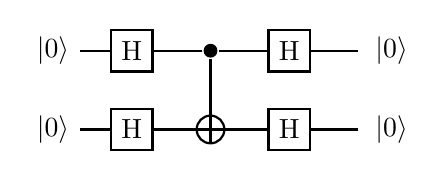
\begin{tikzpicture}[thick]
    %
    % `operator' will only be used by Hadamard (H) gates here.
    % `phase' is used for controlled phase gates (dots).
    % `surround' is used for the background box.
    \tikzstyle{operator} = [draw,fill=white,minimum size=1.5em] 
    \tikzstyle{phase} = [fill,shape=circle,minimum size=5pt,inner sep=0pt]
    \tikzstyle{prod} = [draw,fill=white,shape=circle,minimum size=10pt,inner sep=0pt,path picture={\draw (path picture bounding box.south) -- (path picture bounding box.north) (path picture bounding box.west) -- (path picture bounding box.east);}]]
    \tikzstyle{surround} = [fill=blue!10,thick,draw=black,rounded corners=2mm]
    %
    % Qubits
    \node at (0,0) (q1) {\ket{0}};
    \node at (0,-1) (q2) {\ket{0}};
    %
    % Column 1
    \node[operator] (op11) at (1,0) {H} edge [-] (q1);
    \node[operator] (op21) at (1,-1) {H} edge [-] (q2);
    %
    % Column 3
    \node[phase] (phase11) at (2,0) {} edge [-] (op11);
    \node[prod] (phase12) at (2,-1) {} edge [-] (op21);
    \draw[-] (phase11) -- (phase12);
    %
    % Column 4
    \node[operator] (op23) at (3,0) {H} edge [-] (phase11);
    \node[operator] (op24) at (3,-1) {H} edge [-] (phase12);
    %
    % Column 5
    \node (end1) at (4,0) {} edge [-] (op23);
    \node (end2) at (4,-1) {} edge [-] (op24);
	%    
    % Qubits end
    \node at (4.3,0) (e1) {\ket{0}};
    \node at (4.3,-1) (e2) {\ket{0}};
    %
    \end{tikzpicture}
  }
  \caption{}
\end{figure}

We apply Hadamard transformation to \qb{0}, $H \qb{0} = \asp (\qb{0}+\qb{1})$ as we can see the transformation created \qb{+} in suggested new basis. But we are applying Hadamard on two inputs, therefore the state is afterwards cross product of these two transformed states. Their $\otimes$-product is $\asp (\qb{0}+\qb{1})\otimes \asp (\qb{0}+\qb{1})= \ap (\qb{00} + \qb{01} + \qb{10} + \qb{11})$.

Now we apply C-NOT for this input $\ap (\qb{00} + \qb{01} + \qb{10} + \qb{11})$.

The output can be expressed in matrix C-NOT$\cdot(\ap (\qb{00} + \qb{01} + \qb{10} + \qb{11})$ looks like:
$$
\left( \begin{array}{cccc}
1 & 0 & 0 & 0 \\
0 & 1 & 0 & 0 \\
0 & 0 & 0 & 1 \\
0 & 0 & 1 & 0 \\
\end{array} \right)
\cdot \ap
\left( \begin{array}{cccc}
1 & 0 & 0 & 0 \\
0 & 1 & 0 & 0 \\
0 & 0 & 1 & 0 \\
0 & 0 & 0 & 1 \\
\end{array} \right)
=
\ap
\left( \begin{array}{cccc}
1 & 0 & 0 & 0 \\
0 & 1 & 0 & 0 \\
0 & 0 & 0 & 1 \\
0 & 0 & 1 & 0 \\
\end{array} \right)
$$

We obtained following results: $\ap (\qb{00} + \qb{01} + \qb{10} + \qb{11}) = \ap (\qb{0}(\qb{0} + \qb{1}) + \qb{1}(\qb{0} + \qb{1})) = \ap (\qb{0}+\qb{1})(\qb{0} + \qb{1}))$, but this is exactly the same in new basis \qb{+}\qb{+}.

The last Hadamard transformation create the output of $H \qb{+} = \qb{0}$ for both outputs

So we can see, that for input \qb{+}\qb{+} we really obtain output \qb{+}\qb{+}.

\item The next input configuration is going to be \qb{0},\qb{1}. We already derived Hadamard transformation for the \qb{0}, and for \qb{1} it is H\qb{1} = $\asp (\qb{0} - \qb{1}$, this correspond to the inputs \qb{+}\qb{-}.	

The cross product of inputs \qb{1}\qb{0} is $\asp (\qb{0}+\qb{1})\otimes \asp (\qb{0}-\qb{1})= \ap (\qb{00} - \qb{01} + \qb{10} - \qb{11})$ 

C-NOT operator for such input works as:

$$
\left( \begin{array}{cccc}
1 & 0 & 0 & 0 \\
0 & 1 & 0 & 0 \\
0 & 0 & 0 & 1 \\
0 & 0 & 1 & 0 \\
\end{array} \right)
\cdot \ap
\left( \begin{array}{cccc}
1 & 0 & 0 & 0 \\
0 & -1 & 0 & 0 \\
0 & 0 & 1 & 0 \\
0 & 0 & 0 & -1 \\
\end{array} \right)
=
\ap
\left( \begin{array}{cccc}
1 & 0 & 0 & 0 \\
0 & -1 & 0 & 0 \\
0 & 0 & 0 & -1 \\
0 & 0 & 1 & 0 \\
\end{array} \right)
$$

We obtained following results: $\ap (\qb{00} - \qb{01} - \qb{10} + \qb{11}) = \ap (\qb{0}(\qb{0} - \qb{1}) - \qb{1}(\qb{0} + \qb{1})) = \ap (\qb{0}-\qb{1})(\qb{0}-\qb{1}))$, but this is exactly the same in new basis \qb{-} and \qb{-}. So for input \qb{+}\qb{-} the result is \qb{-}\qb{-} which transformed into standard basis is \qb{1}\qb{1}.

\begin{figure}[h]
  \centerline{
    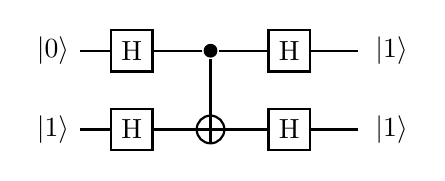
\begin{tikzpicture}[thick]
    %
    % `operator' will only be used by Hadamard (H) gates here.
    % `phase' is used for controlled phase gates (dots).
    % `surround' is used for the background box.
    \tikzstyle{operator} = [draw,fill=white,minimum size=1.5em] 
    \tikzstyle{phase} = [fill,shape=circle,minimum size=5pt,inner sep=0pt]
    \tikzstyle{prod} = [draw,fill=white,shape=circle,minimum size=10pt,inner sep=0pt,path picture={\draw (path picture bounding box.south) -- (path picture bounding box.north) (path picture bounding box.west) -- (path picture bounding box.east);}]]
    \tikzstyle{surround} = [fill=blue!10,thick,draw=black,rounded corners=2mm]
    %
    % Qubits
    \node at (0,0) (q1) {\ket{0}};
    \node at (0,-1) (q2) {\ket{1}};
    %
    % Column 1
    \node[operator] (op11) at (1,0) {H} edge [-] (q1);
    \node[operator] (op21) at (1,-1) {H} edge [-] (q2);
    %
    % Column 3
    \node[phase] (phase11) at (2,0) {} edge [-] (op11);
    \node[prod] (phase12) at (2,-1) {} edge [-] (op21);
    \draw[-] (phase11) -- (phase12);
    %
    % Column 4
    \node[operator] (op23) at (3,0) {H} edge [-] (phase11);
    \node[operator] (op24) at (3,-1) {H} edge [-] (phase12);
    %
    % Column 5
    \node (end1) at (4,0) {} edge [-] (op23);
    \node (end2) at (4,-1) {} edge [-] (op24);
	%    
    % Qubits end
    \node at (4.3,0) (e1) {\ket{1}};
    \node at (4.3,-1) (e2) {\ket{1}};
    %
    \end{tikzpicture}
  }
  \caption{}
\end{figure}


\item We already covered all basic Hadamard transformations so this part will only briefly describes the process of computation. 
\begin{itemize}
\item For input \qb{1}\qb{0} after Hadamard transformation the input for C-NOT is \qb{-}$\otimes$\qb{+} which is $\asp (\qb{0}-\qb{1})\otimes \asp (\qb{0}+\qb{1})= \ap (\qb{00} + \qb{01} - \qb{10} - \qb{11})$
\item C-NOT$\cdot\qb{-}\otimes\qb{+}$ 
$$
\left( \begin{array}{cccc}
1 & 0 & 0 & 0 \\
0 & 1 & 0 & 0 \\
0 & 0 & 0 & 1 \\
0 & 0 & 1 & 0 \\
\end{array} \right)
\cdot \ap
\left( \begin{array}{cccc}
1 & 0 & 0 & 0 \\
0 & 1 & 0 & 0 \\
0 & 0 & -1 & 0 \\
0 & 0 & 0 & -1 \\
\end{array} \right)
=
\ap
\left( \begin{array}{cccc}
1 & 0 & 0 & 0 \\
0 & 1 & 0 & 0 \\
0 & 0 & 0 & -1 \\
0 & 0 & -1 & 0 \\
\end{array} \right)
$$

\item Result $\ap (\qb{00} + \qb{01} - \qb{10} - \qb{11}) = \ap (\qb{0}-\qb{1}) (\qb{0}+\qb{1})$ is the same as input \qb{-}\qb{+}.
\item The Hadamard transformation at the end give us results in standard basis \qb{1} and \qb{0}.
\end{itemize}
\begin{figure}[h]
  \centerline{
    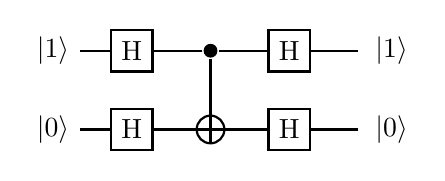
\begin{tikzpicture}[thick]
    %
    % `operator' will only be used by Hadamard (H) gates here.
    % `phase' is used for controlled phase gates (dots).
    % `surround' is used for the background box.
    \tikzstyle{operator} = [draw,fill=white,minimum size=1.5em] 
    \tikzstyle{phase} = [fill,shape=circle,minimum size=5pt,inner sep=0pt]
    \tikzstyle{prod} = [draw,fill=white,shape=circle,minimum size=10pt,inner sep=0pt,path picture={\draw (path picture bounding box.south) -- (path picture bounding box.north) (path picture bounding box.west) -- (path picture bounding box.east);}]]
    \tikzstyle{surround} = [fill=blue!10,thick,draw=black,rounded corners=2mm]
    %
    % Qubits
    \node at (0,0) (q1) {\ket{1}};
    \node at (0,-1) (q2) {\ket{0}};
    %
    % Column 1
    \node[operator] (op11) at (1,0) {H} edge [-] (q1);
    \node[operator] (op21) at (1,-1) {H} edge [-] (q2);
    %
    % Column 3
    \node[phase] (phase11) at (2,0) {} edge [-] (op11);
    \node[prod] (phase12) at (2,-1) {} edge [-] (op21);
    \draw[-] (phase11) -- (phase12);
    %
    % Column 4
    \node[operator] (op23) at (3,0) {H} edge [-] (phase11);
    \node[operator] (op24) at (3,-1) {H} edge [-] (phase12);
    %
    % Column 5
    \node (end1) at (4,0) {} edge [-] (op23);
    \node (end2) at (4,-1) {} edge [-] (op24);
	%    
    % Qubits end
    \node at (4.3,0) (e1) {\ket{1}};
    \node at (4.3,-1) (e2) {\ket{0}};
    %
    \end{tikzpicture}
  }
  \caption{}
\end{figure}

\item Only briefly the last case:
\begin{itemize}
\item For input \qb{1}\qb{1} after Hadamard transformation the input for C-NOT is \qb{1}$\otimes$\qb{1} which is $\asp (\qb{0}-\qb{1})\otimes \asp (\qb{0}-\qb{1})= \ap (\qb{00} - \qb{01} - \qb{10} + \qb{11})$
\item C-NOT$\cdot\qb{-}\otimes\qb{-}$ 
$$
\left( \begin{array}{cccc}
1 & 0 & 0 & 0 \\
0 & 1 & 0 & 0 \\
0 & 0 & 0 & 1 \\
0 & 0 & 1 & 0 \\
\end{array} \right)
\cdot \ap
\left( \begin{array}{cccc}
1 & 0 & 0 & 0 \\
0 & -1 & 0 & 0 \\
0 & 0 & -1 & 0 \\
0 & 0 & 0 & 1 \\
\end{array} \right)
=
\ap
\left( \begin{array}{cccc}
1 & 0 & 0 & 0 \\
0 & -1 & 0 & 0 \\
0 & 0 & 0 & 1 \\
0 & 0 & -1 & 0 \\
\end{array} \right)
$$

\item Result $\ap (\qb{00} - \qb{01} + \qb{10} - \qb{11}) = \ap (\qb{0}+\qb{1}) (\qb{0}-\qb{1})$ is \qb{+}\qb{-}.
\item The Hadamard transformation at the end give us results in standard basis \qb{0} and \qb{1}.

\begin{figure}[h!]
  \centerline{
    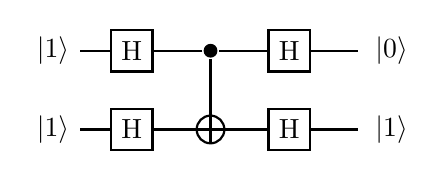
\begin{tikzpicture}[thick]
    %
    % `operator' will only be used by Hadamard (H) gates here.
    % `phase' is used for controlled phase gates (dots).
    % `surround' is used for the background box.
    \tikzstyle{operator} = [draw,fill=white,minimum size=1.5em] 
    \tikzstyle{phase} = [fill,shape=circle,minimum size=5pt,inner sep=0pt]
    \tikzstyle{prod} = [draw,fill=white,shape=circle,minimum size=10pt,inner sep=0pt,path picture={\draw (path picture bounding box.south) -- (path picture bounding box.north) (path picture bounding box.west) -- (path picture bounding box.east);}]]
    \tikzstyle{surround} = [fill=blue!10,thick,draw=black,rounded corners=2mm]
    %
    % Qubits
    \node at (0,0) (q1) {\ket{1}};
    \node at (0,-1) (q2) {\ket{1}};
    %
    % Column 1
    \node[operator] (op11) at (1,0) {H} edge [-] (q1);
    \node[operator] (op21) at (1,-1) {H} edge [-] (q2);
    %
    % Column 3
    \node[phase] (phase11) at (2,0) {} edge [-] (op11);
    \node[prod] (phase12) at (2,-1) {} edge [-] (op21);
    \draw[-] (phase11) -- (phase12);
    %
    % Column 4
    \node[operator] (op23) at (3,0) {H} edge [-] (phase11);
    \node[operator] (op24) at (3,-1) {H} edge [-] (phase12);
    %
    % Column 5
    \node (end1) at (4,0) {} edge [-] (op23);
    \node (end2) at (4,-1) {} edge [-] (op24);
	%    
    % Qubits end
    \node at (4.3,0) (e1) {\ket{0}};
    \node at (4.3,-1) (e2) {\ket{1}};
    %
    \end{tikzpicture}
  }
  \caption{}
\end{figure}
\end{itemize}
\item In the previous bullets we have show that the C-NOT gate behaves for the the \qb{+},\qb{-} basis as expected, i.e. the roles of control and target are reversed. We can see that because of this and because of the Hadamard transformation before and after the C-NOT gate this circuit behaves like this:
\begin{figure}[h!]
\centering
\begin{tabular}{|c|c|}
\hline
input & output \\ \hline
\qb{0}\qb{0} & \qb{0}\qb{0} \\ \hline
\qb{0}\qb{1} & \qb{1}\qb{1} \\ \hline
\qb{1}\qb{0} & \qb{1}\qb{0} \\ \hline
\qb{1}\qb{1} & \qb{0}\qb{1} \\ \hline
\end{tabular}
\end{figure}

which is exactly same output as we would obtain from inverted C-NOT gate with the fist bit as a target and the second as a control:

\begin{figure}[h!]
  \centerline{
    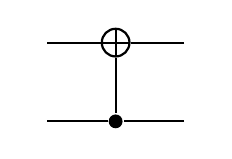
\begin{tikzpicture}[thick]
    %
    % `operator' will only be used by Hadamard (H) gates here.
    % `phase' is used for controlled phase gates (dots).
    % `surround' is used for the background box.
    \tikzstyle{operator} = [draw,fill=white,minimum size=1.5em] 
    \tikzstyle{phase} = [fill,shape=circle,minimum size=5pt,inner sep=0pt]
    \tikzstyle{prod} = [draw,fill=white,shape=circle,minimum size=10pt,inner sep=0pt,path picture={\draw (path picture bounding box.south) -- (path picture bounding box.north) (path picture bounding box.west) -- (path picture bounding box.east);}]]
    \tikzstyle{surround} = [fill=blue!10,thick,draw=black,rounded corners=2mm]
    %
    % Qubits
    \node (s1) at (0,0) {};
    \node (s2) at (0,-1) {};
    %
    % Column 3
    \node[prod] (phase11) at (1,0) {} edge [-] (s1);
    \node[phase] (phase12) at (1,-1) {} edge [-] (s2);
    \draw[-] (phase11) -- (phase12);
    %
    % Column 5
    \node (end1) at (2,0) {} edge [-] (phase11);
    \node (end2) at (2,-1) {} edge [-] (phase12);
    %
    \end{tikzpicture}
  }
  \caption{}
\end{figure}
\end{enumerate}
\end{document}